%%%%%%%%%%%%%%%%%%%%%%%%%%% asme2ej.tex %%%%%%%%%%%%%%%%%%%%%%%%%%%%%%%
% Template for producing ASME-format journal articles using LaTeX    %
% Written by   Harry H. Cheng, Professor and Director                %
%              Integration Engineering Laboratory                    %
%              Department of Mechanical and Aeronautical Engineering %
%              University of California                              %
%              Davis, CA 95616                                       %
%              Tel: (530) 752-5020 (office)                          %
%                   (530) 752-1028 (lab)                             %
%              Fax: (530) 752-4158                                   %
%              Email: hhcheng@ucdavis.edu                            %
%              WWW:   http://iel.ucdavis.edu/people/cheng.html       %
%              May 7, 1994                                           %
% Modified: February 16, 2001 by Harry H. Cheng                      %
% Modified: January  01, 2003 by Geoffrey R. Shiflett                %
% Butchered: October 15, 2014 by John Karasinski                     %
% Use at your own risk, send complaints to /dev/null                 %
%%%%%%%%%%%%%%%%%%%%%%%%%%%%%%%%%%%%%%%%%%%%%%%%%%%%%%%%%%%%%%%%%%%%%%

%%% use twocolumn and 10pt options with the asme2ej format
\documentclass[twocolumn,10pt]{asme2ej}

\usepackage{epsfig} %% for loading postscript figures
\usepackage{amsmath}
\usepackage{graphicx}
\usepackage{grffile}
\usepackage{pdfpages}
\usepackage{algpseudocode}

% Default fixed font does not support bold face
\DeclareFixedFont{\ttb}{T1}{txtt}{bx}{n}{12} % for bold
\DeclareFixedFont{\ttm}{T1}{txtt}{m}{n}{12}  % for normal

% Custom colors
\usepackage{color}
% \definecolor{deepblue}{rgb}{0,0,0.5}
% \definecolor{deepred}{rgb}{0.6,0,0}
% \definecolor{deepgreen}{rgb}{0,0.5,0}

\usepackage{listings}

% Python style for highlighting
% \newcommand\pythonstyle{\lstset{
% language=Python,
% basicstyle=\ttm,
% otherkeywords={self},             % Add keywords here
% keywordstyle=\ttb\color{deepblue},
% emph={MyClass,__init__},          % Custom highlighting
% emphstyle=\ttb\color{deepred},    % Custom highlighting style
% stringstyle=\color{deepgreen},
% frame=tb,                         % Any extra options here
% showstringspaces=false            %
% }}

\definecolor{mygreen}{rgb}{0,0.6,0}
\definecolor{mygray}{rgb}{0.5,0.5,0.5}
\definecolor{mymauve}{rgb}{0.58,0,0.82}

\lstset{ %
  backgroundcolor=\color{white},   % choose the background color; you must add \usepackage{color} or \usepackage{xcolor}
  basicstyle=\ttfamily\footnotesize, % the size of the fonts that are used for the code
  breakatwhitespace=false,         % sets if automatic breaks should only happen at whitespace
  % breaklines=true,                 % sets automatic line breaking
  captionpos=b,                    % sets the caption-position to bottom
  commentstyle=\color{mygreen},    % comment style
  deletekeywords={...},            % if you want to delete keywords from the given language
  escapeinside={\%*}{*)},          % if you want to add LaTeX within your code
  extendedchars=true,              % lets you use non-ASCII characters; for 8-bits encodings only, does not work with UTF-8
  frame=single,                    % adds a frame around the code
  keepspaces=true,                 % keeps spaces in text, useful for keeping indentation of code (possibly needs columns=flexible)
  columns=flexible,
  keywordstyle=\color{blue},       % keyword style
  language=Python,                 % the language of the code
  morekeywords={*,...},            % if you want to add more keywords to the set
  numbers=left,                    % where to put the line-numbers; possible values are (none, left, right)
  numbersep=5pt,                   % how far the line-numbers are from the code
  numberstyle=\tiny\color{mygray}, % the style that is used for the line-numbers
  rulecolor=\color{black},         % if not set, the frame-color may be changed on line-breaks within not-black text (e.g. comments (green here))
  showspaces=false,                % show spaces everywhere adding particular underscores; it overrides 'showstringspaces'
  showstringspaces=false,          % underline spaces within strings only
  showtabs=false,                  % show tabs within strings adding particular underscores
  stepnumber=1,                    % the step between two line-numbers. If it's 1, each line will be numbered
  stringstyle=\color{mymauve},     % string literal style
  tabsize=4,                       % sets default tabsize to 2 spaces
  % title=\lstname                   % show the filename of files included with \lstinputlisting; also try caption instead of title
}

\title{Case Study \# 3: Structural Analysis: Perforated Plate in Tension}

\author{John Karasinski
    \affiliation{
  Graduate Student Researcher\\
  Center for Human/Robotics/Vehicle Integration and Performance\\
  Department of Mechanical and Aerospace Engineering\\
  University of California\\
  Davis, California 95616\\
    Email: karasinski@ucdavis.edu
    }
}

\begin{document}
\maketitle

%%%%%%%%%%%%%%%%%%%%%%%%%%%%%%%%%%%%%%%%%%%%%%%%%%%%%%%%%%%%%%%%%%%%%%
\section{Problem Description}
This case study involves a linear-elastic, steady-state stress analysis on a square plate with a circular hole at its center. The plate dimensions are: side length $x = 4$m and radius $R = 0.5$m. It is loaded with a uniform traction of $\sigma = 10$kPa over its left and right faces as can be seen in Figure~\ref{geometry}. A mesh sensitivity study is performd for a plate with side length $x = 4$m, and an effect of the plate length study is performed for plates of length $x = 3$m, 4m, 5m, and 100m.

The stress normal to the vertical plane of symmetry is calculated for each case, and the results are compared to the analytical solution:
\begin{equation}
(\sigma_{xx})_{x=0} \left\{ \begin{array}{lll}
        \mbox{$\sigma(1+\frac{R^2}{2Y^2}+\frac{3R^4}{2y^4}) $} & \mbox{for } &|y| \geq R \\
        \mbox{$0$} & \mbox{for } &|y| < R \end{array} \right.
\label{vertical_stress}
\end{equation}

A Python script was created to automatically generate the configuration files, calculate the resulting steady-state stress through the plate using OpenFOAM, and plot the results for both the sensitivity and plate length studies. This script can be seen in the Appendix.

\begin{figure}[b]
\begin{center}
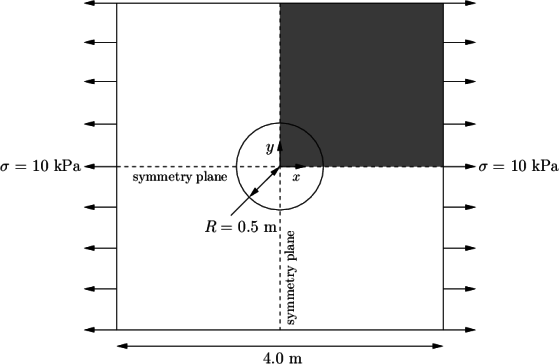
\includegraphics[width=0.5\textwidth]{figure/user144x.png}
\caption{Geometry of the plate with a hole}
\label{geometry}
\end{center}
\end{figure}

%%%%%%%%%%%%%%%%%%%%%%%%%%%%%%%%%%%%%%%%%%%%%%%%%%%%%%%%%%%%%%%%%%%%%%
\section{Numerical Solution Approach}
 Two symmetry planes can be identified for this geometry and therefore the solution domain need only cover a quarter of the geometry, shown by the shaded area in Figure~\ref{geometry}. The quarter plate is then broken into five blocks of varying sizes, as can be seen in Figure~\ref{blocks}. These blocks have a characteristic number of points, $n$. Blocks 0 and 1 consist of $n$ by $n$ points, block 2 consists of $2n$ by $n$ points, block 3 consists of $2n$ by $2n$ points, and block 4 consists of $n$ by $2n$ points. The mesh is generated with OpenFOAM's `blockMesh' and Figure~\ref{mesh} shows the resulting mesh for $n = 10$.

 The mesh sensity study looks at meshes of $n = 10, 100, $ and $1000$ and a plate width of $x = 4$m. The effect of plate length study looks at plate lengths of $x = 3$m, 4m, 5m, and 100m with a mesh of $n = 10$. Once the meshes have been generated, OpenFOAM's `solidDisplacementFoam' solver runs the simulation, and $\sigma_{xx}$ is calculated and sampled by the OpenFOAM commands `foamCalc components sigma' and `sample'.

\begin{figure}[tb]
\begin{center}
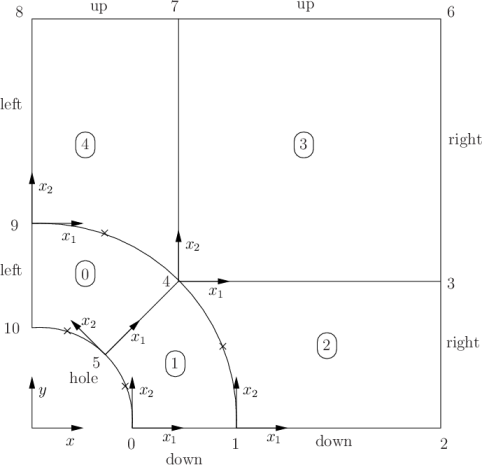
\includegraphics[width=0.5\textwidth]{figure/user149x.png}
\caption{Block structure of the mesh for the plate with a hole}
\label{blocks}
\end{center}
\end{figure}

\begin{figure}[tb]
\begin{center}
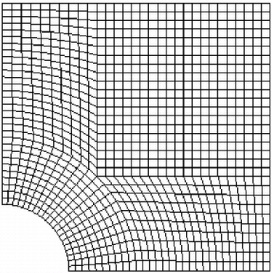
\includegraphics[width=0.5\textwidth]{figure/user152x.png}
\caption{Mesh of the hole in a plate problem with $n = 10$}
\label{mesh}
\end{center}
\end{figure}

%%%%%%%%%%%%%%%%%%%%%%%%%%%%%%%%%%%%%%%%%%%%%%%%%%%%%%%%%%%%%%%%%%%%%%
\section{Results Discussion}
\noindent Mesh sensitivity study\\
Selected key results for the base case\\
Effect of the plate length study\\
Summary of the difficulties that you have encountered in running the various cases and how you have addressed them.\\

%%%%%%%%%%%%%%%%%%%%%%%%%%%%%%%%%%%%%%%%%%%%%%%%%%%%%%%%%%%%%%%%%%%%%%
\section{Conculsion}

%%%%%%%%%%%%%%%%%%%%%%%%%%%%%%%%%%%%%%%%%%%%%%%%%%%%%%%%%%%%%%%%%%%%%%
\clearpage
\onecolumn
\appendix       %%% starting appendix
\section*{Appendix A: Python Code}

\lstinputlisting[language=Python]{../code/CaseStudy3.py}

%%%%%%%%%%%%%%%%%%%%%%%%%%%%%%%%%%%%%%%%%%%%%%%%%%%%%%%%%%%%%%%%%%%%%%
\end{document}
